\documentclass{article}

% set font encoding for PDFLaTeX or XeLaTeX
\usepackage{ifxetex}
\ifxetex
  \usepackage{fontspec}
\else
  \usepackage[T1]{fontenc}
  \usepackage[utf8]{inputenc}
  \usepackage{lmodern}
  \usepackage{graphicx}
\fi



% used in maketitle

\title{Reporte Actividad 3}
\author{José Burruel}
\date{Marzo 4 del 2018}

\newpage

\begin{document}
\maketitle{ Relación entre altura y características atmosféricas}

\section{Introducción}
En esta actividad vimos un poco más a fondo el analisis de datos con Panda y Matplotlib de Python mientras trabajamos datos de atmósferas proporcionados por la Universidad de Wyoming.

\section{Fundamentos}
Los elementos fundamentales que uno debe conocer para poder enteder los resultados que vamos a mostrar en unos momentos son de variables físicas tangibles por sensores en alturas altas, como por ejemplo:

    \begin{enumerate}
        \item{Altura}
        \item{Presión}
        \item{Temperatura}
        \item{Velocidades del viento}
        \item{Humedad Relativa}
    \end{enumerate}

También se deberá comprender los conceptos de las distintas capas de la atmósfera.

En esta actividad se analizará el cambio en estas variables con respecto a la altura en la que se tomaron los datos en la atmósfera.

\section{Analisis de Datos}
El procedimiento realizado fue, primeramente, tomar los datos de los sondeos atmosféricos de la Universidad de Wyoming, y descargar la lista de los datos en archivo txt, editado en Emacs, y procesados directamente en Jupyter Notebook para poder trabajar con Python. Se tomaron datos del 22 de Junio y el 22 de Diciembre para ver si existe un cambio directo entre la fecha también.
Siguiente, en Python se utilizó el paquete de Panda para el análisis y Matplotlib para poder hacer las gráficas en función de la altura que presentaremos a continuacion.

\newpage

\section{Resultados}

\begin{figure}
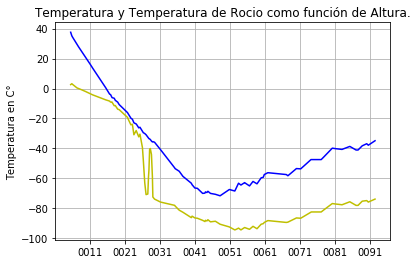
\includegraphics[width=\linewidth]{TemperaturasJun.png}
\caption{Grafica de Temperatura contra altura de Junio del 2017}
\centering
\end{figure}

\begin{figure}
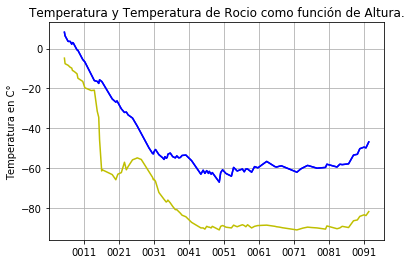
\includegraphics[width=\linewidth]{TemperaturasDic.png}
\caption{Grafica de Temperatura contra Altura de Diciembre del 2017}
\end{figure}

\begin{figure}
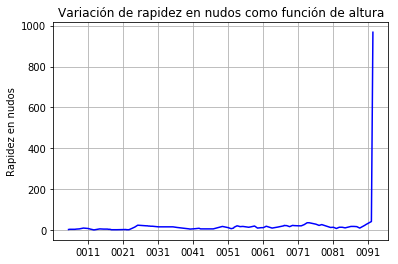
\includegraphics[width=\linewidth]{RapidezJun.png}
\caption{Grafica de Rapidez en nudos contra altura de Junio del 2017}
\end{figure}

\begin{figure}
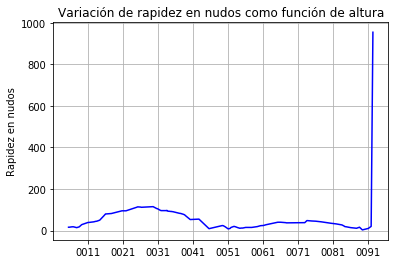
\includegraphics[width=\linewidth]{RapidezDic.png}
\caption{Grafica de Rapidez de Diciembre del 2017}
\end{figure}

\begin{figure}
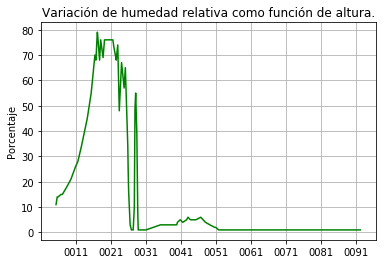
\includegraphics[width=\linewidth]{HumedadJun.png}
\caption{Grafica de Humedad contra Altura de Junio del 2017}
\end{figure}

\begin{figure}
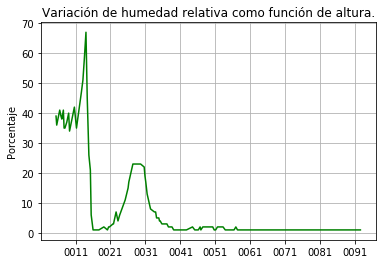
\includegraphics[width=\linewidth]{HumedadDic.png}
\caption{Grafica de Humedad contra Altura de Diciembre del 2017}
\end{figure}

\newpage

\section{Conclusión}
Primero que nada, podemos ver que en el mes de Junio no se tomaron muchos datos por las sondas de la Universidad de Wyoming, pero lo que podemos concluir después de éste simple análisis es que las variables físicas sí son afectadas por la altura de las capas de la atmósfera y que cada una de ellas, diferentes unas de las otras, también tienen diferencias en estas variables estudiadas.

\section{Apéndice}
\subsection{¿Cuál es tu opinión general de esta actividad?}
Nos da una mejor idea de como se aplica éste lenguaje de programación en el estudio científico.
\subsection{¿Qué fue lo que más te agradó? ¿Lo que menos te agradó?}
Lo que más me gustó es lo fácil que se puede hacer una gráfica con Matplotlib.
Lo que menos me gustó fue hacer el reporte.
\subsection{¿Que consideras que aprendiste en esta actividad?}
Pues, como dije en la primera pregunta, que está curado que nos da una idea del trabajo científico que se puede realizar con las herramientas proporcionadas por el lenguaje de programación Python.
\subsection{¿Qué le faltó? ¿O le sobró? }
Se me hace que le falta un poco más de insight a la parte de clase dada por el profesor, ya que, en su mayoría, es mucho "Ahí están las herramientas, dense", cuando habemos personas que nos gustaría un poco más tener esa ayuda de enseñanza teórica por un experto en el tema.
\subsection{¿Que mejoras sugieres a la actividad?}
Lo mismo que dije arriba :P




\end{document}
